\documentclass[9pt,twocolumn,twoside]{../../styles/osajnl}
\usepackage{fancyvrb}
\journal{i524} 

\title{MongoDB}

\author[1,*]{Nandita Sathe}

\affil[1]{School of Informatics and Computing, Bloomington, IN 47408, U.S.A.}

\affil[*]{Corresponding author: nsathe@iu.edu}

\dates{paper-1, \today}

\ociscodes{I524, MongoDB, NoSQL}

\doi{\url{https://github.com/cloudmesh/sp17-i524/raw/master/paper1/S17-IO-3017/report.pdf}}


\begin{abstract}
MongoDB is a NoSQL database. Instead of using tables and rows as in relational databases, MongoDB is built on an architecture of collections and documents. Documents comprise sets of key-value pairs and are the basic unit of data in MongoDB. Collections contain sets of documents and function as the equivalent of relational database tables. MongoDB database is used when data size is expected to be huge and schema is not stable.
\newline
\end{abstract}

\setboolean{displaycopyright}{true}

\begin{document}

\maketitle

\section{Introduction}

MongoDB is a non-RDBMS key-value data store. The data to be stored does not necessarily have to follow a fixed schema. In relational database data is stored primarily in tables. In NoSQL database like MongoDB data is stored in collections. A collection acts as a container for a 'Document'. A Document is equivalent to a row of a table. The data in MongoDB Document is stored in JSON array like data structure. The database also supports large volume of data storage and offers very high data insert speed due to its schema-less design \cite{paper-mongo1}. 

\section{Infrastructure and Performance}

Following sections discuss key deployment considerations.

\subsection{Working set size}

The set of data and indexes that are accessed most frequently during normal operations is called the working set. Working set resides in memory rather than on disk to ensure low latency database operations. Ideally working set should fit into RAM. Before MongoDB deployment it is necessary to assess the working set size based on the size of data and kind of operations that will be performed on data, so that adequate RAM size can be determined. Page faults occur in case working set size exceeds the available RAM. In this case either the RAM size should be increased or sharding should be done (see Section 2.4).   

\subsection {Storage and Disk I/O}

If working set size is far larger than any available memory, then selecting the proper disk type for deployment is important. Local disks should be used as far as possible as the network storage can cause high latency and poor performance.

\subsection {CPU Selection}

MongoDB performance is typically not CPU-bound. As MongoDB rarely encounters workloads and is able to leverage large numbers of cores, it is preferable to have servers with faster clock speeds than numerous cores with slower clock speeds \cite{www-mongo4}.

\subsection {Sharding}

MongoDB partitions data across servers using a technique called Sharding. Balancing of data across shards is automatic, and shards can be added and removed without taking the database offline \cite{www-mongo3}. Sharding allows the database to scale out on hardware deployed on-premises or in the cloud, enabling almost unlimited growth with higher throughput and lower latency than relational databases \cite{www-mongo5}. Figure \ref{fig:figure1} shows scaling of database.

\begin{figure}[htbp]
\centering
\fbox{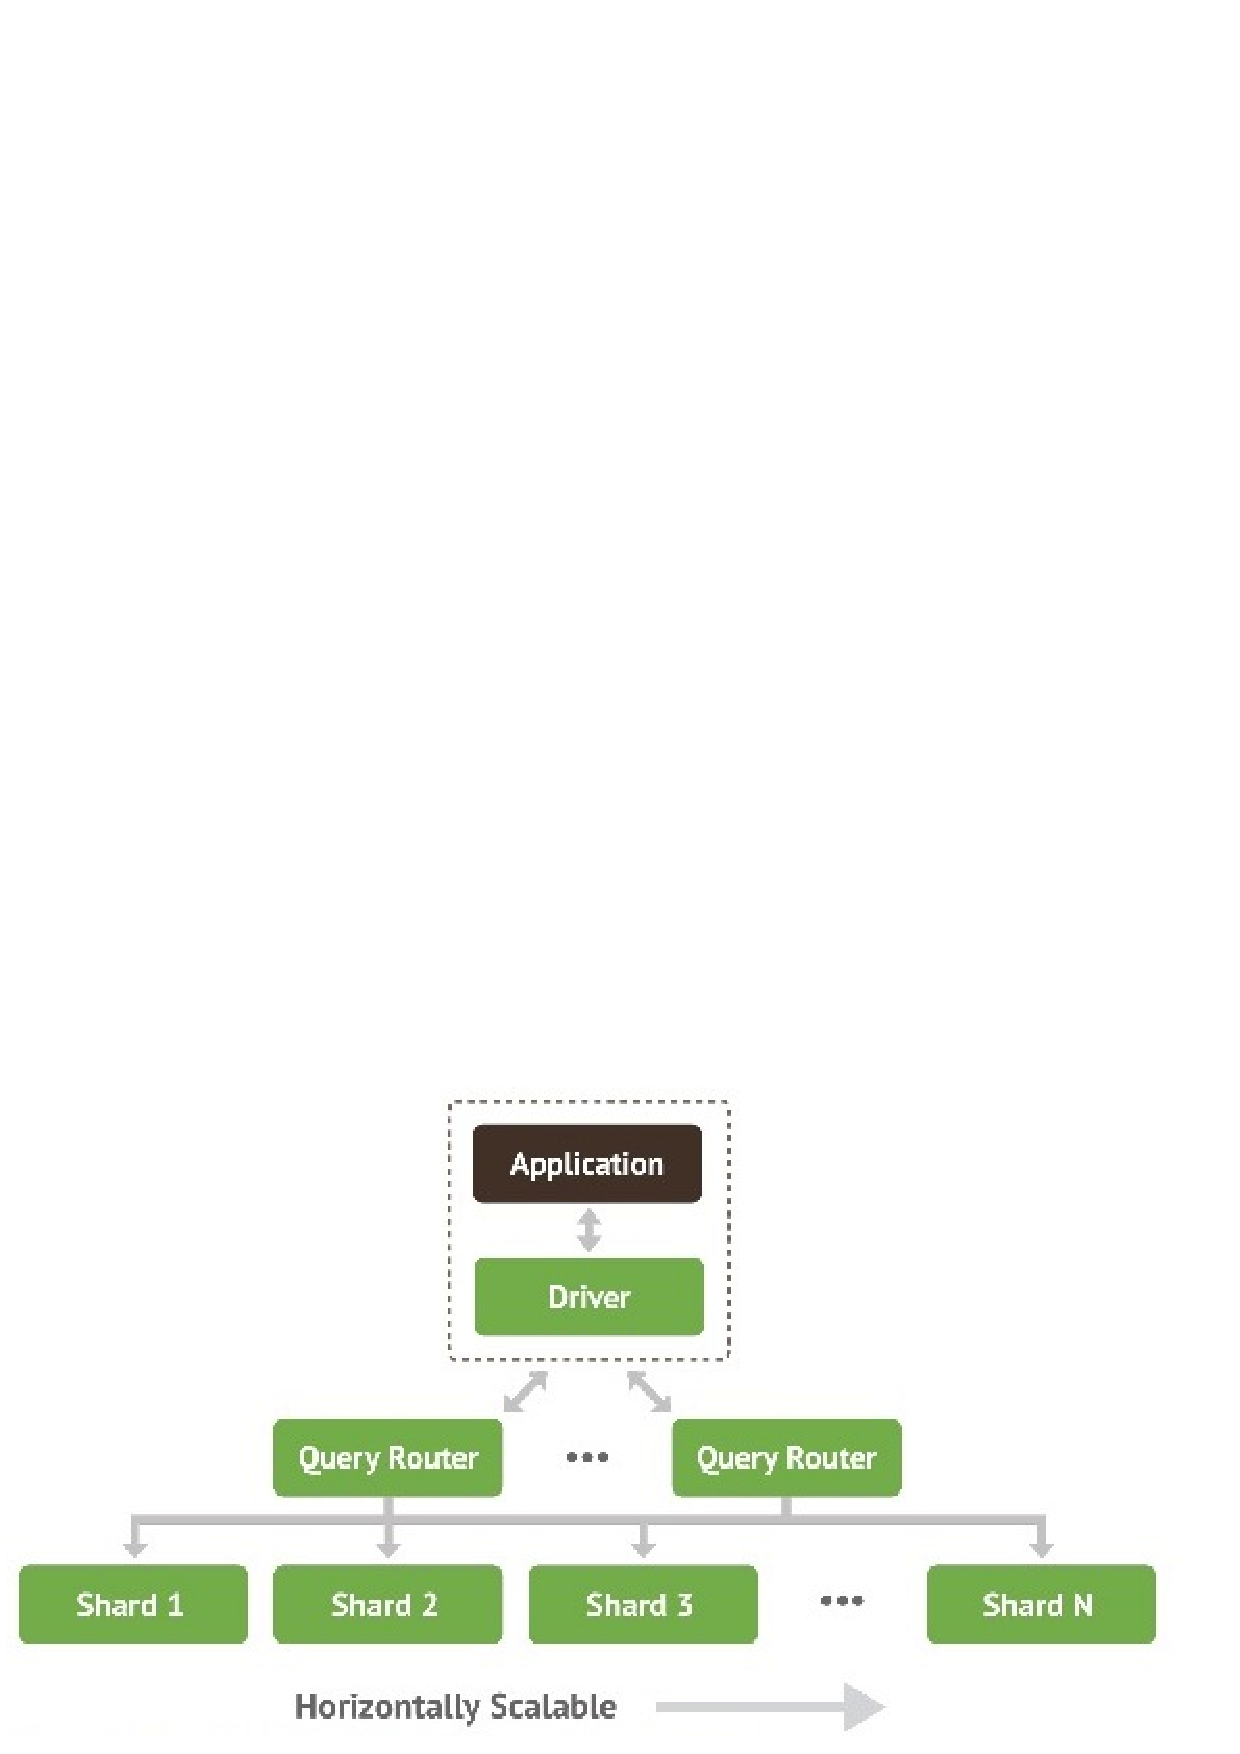
\includegraphics[width=\linewidth]{images/figure1}}
\caption{MongoDB Auto-sharding \cite{www-mongo4}.} 
\label{fig:figure1}
\end{figure}

Users should consider deploying a sharded MongoDB cluster in the following situations \cite{www-mongo4}:

{\bfseries RAM Limitation:} If the working set size is expected to exceed the capacity of the maximum amount of RAM in the system.

{\bfseries Disk I/O Limitation:} If the system has a large amount of
write activity, and the operating system cannot write data fast enough
to meet demand.

{\bfseries Storage Limitation:} If the data set approaches or exceeds the
storage capacity of a single node in the system.

\subsection {Replication}

MongoDB maintains multiple copies of data called replica sets using native replication. A replica set consists of multiple replicas. At any given time, one member acts as the primary replica set member and the other members act as secondary replica set members. Reads and writes are issued to a primary copy of the data. If the primary member fails for any reason (e.g., hardware failure, network partition), one of the secondary members is automatically elected to primary and begins to process all writes \cite{www-mongo6}.

Figure \ref{fig:figure2} shows replica sets maintained by MongoDB.

\begin{figure}[htbp]
\centering
\fbox{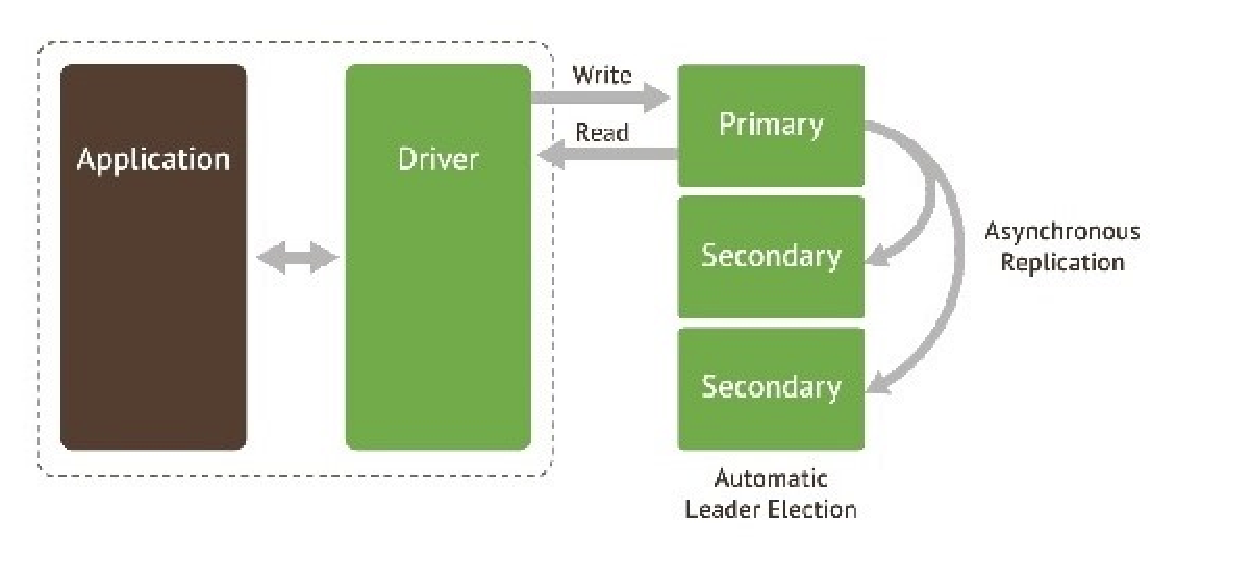
\includegraphics[width=\linewidth]{images/figure2}}
\caption{MongoDB replica sets \cite{www-mongo4}.} 
\label{fig:figure2}
\end{figure}

\subsection {Indexing}

Indexes are a crucial mechanism for optimizing system performance and scalability. MongoDB includes support for many types of secondary indexes that can be declared on any field in the document, including fields within arrays:

One can define compound, unique, array, partial, TTL, geospatial, sparse, hash and text indexes to optimize for multiple query patterns, multi-structured data types and constraints.

Index intersection enables MongoDB to use more than one index to optimize an ad-hoc query at run-time \cite{www-mongo5}.
    
\section{Features}

These are main features of MongoDB.\cite{www-mongo11}
\begin{itemize}
\item General purpose database, almost as fast as the key:value NoSQL type.
\item Scalability: (from a standalone server to distributed
  architectures of huge clusters). This allows us to shard our
  database transparently across all our shards. This increases the
  performance of our data processing.
\item Aggregation: batch data processing and aggregate calculations
  using native MongoDB operations.
\item Load Balancing: automatic data movement across different shards
  for load balancing. The balancer decides when to migrate the data
  and the destination Shard, so they are evenly distributed among all
  servers in the cluster. Each shard stores the data for a selected
  range of our collection according to a partition key.
\item Native Replication: syncing data across all the servers at the
  replica set.
\item Security: authentication, authorization, etc.
\item Advanced users management.
\item Automatic failover: automatic election of a new primary when it
  has gone down.
\item Zero downtime upgrades.
\item There are no bottlenecks processing large volumes of data.
\item MongoDB uses JSON objects to store and transmit information.
\item We can do queries and geospatial operations in 2D and 3D.
\item We can utilize Map-Reduce for information processing using
  JavaScript functions at the server side.
\item JavaScript execution: Ability to store JavaScript functions on
  the server for queries and aggregation functions
\item MongoDB Management Service. (MMS) is a powerful web tool that
  allows us tracking our databases and our machines and also backing
  up our data.
\item Monitoring: MMS tracks the database and hardware metrics for managing MongoDB deployment. Performance is visualized in a rich web console to help optimize your deployment. Discover issues via custom alerts before MongoDB instance will be affected.
\item Backup: Continuous backup with point-in-time recovery of replica sets and sharded clusters. Multiple copies of every backup are archived across data centers (geographically distributed and fault-tolerant)

\end{itemize}

\section{MongoDB for BigData Analytics}

At the top level there are 3 Vs that define BigData - Volume, Variety and Velocity. MongoDB supports storage of high volume of data which is complex in nature. Its dynamic schema provides a major advantage for businesses that need to ingest, store, and process rapidly evolving data streams from new sources. The term velocity refers to high and volatile inbound data, faster query at low latency. MongoDB is designed to support insertion of high volume of data in less time and faster response to query \cite{www-mongo1}.

For data analysis one can utilise built-in aggregation functionality provided by MongoDB. In case of more complex data analytics one can leverage Hadoop and Apache Spark framework. To be able to connect efficiently to MongoDB Hadoop and Spark connectors are available and can be configured easily. In this scenario data is pulled from MongoDB and complex processing is performed in Hadoop/Spark, output of the processing can then be written back to MongoDB for later querying and ad-hoc analysis.

\section{MongoDB Use Cases}

Some of the common MongoDB use cases involve operational intelligence, Internet of Things, content management and real-time analytics. Following are some of the MongoDB customers \cite{www-mongo14}.

BOSCH: The Bosch IoT Suite is a cloud-enabled software package for developing applications in the Internet of Things (IoT). Bosch has built its Internet of Things suite on MongoDB. MongoDB has been used to manage massive volume and unstructured nature of IoT data and perform real-time analytics.

Aadhar: India’s Unique Identification project, Aadhar, maintains biometrics database. Aadhar is in the process of capturing demographic and biometric data of over 1.2 billion residents. Aadhar has used MongoDB as one of its databases to store this huge amount of data. 

MetLife: MetLife uses MongoDB for its customer service application called 'The Wall'. It provides a consolidated view of MetLife customers, including policy details and transactions. 

eBay: eBay has a number of projects running on MongoDB for search suggestions, metadata storage, cloud management and merchandizing categorization.

\section{Licensing}

MongoDB database server and tools are available under GNU AGPL v3.0.

\section{Educational Material}

To get started on learning MongoDB, following resources can prove helpful.

\begin{itemize}
\item Helpful tutorials for beginner developers - https://www.tutorialspoint.com/mongodb/

\item MongoDB's documents. You will find reference material for everything here - https://docs.mongodb.com/v3.2/\#getting-started

\item Fixed schedule course on MongoDB - https://university.mongodb.com/

\item MongoDB course specifically for Data Scientists - https://www.udacity.com/course/data-wrangling-with-mongodb--ud032

\end{itemize}

\section{Comparison}

There are various alternatives for MongoDB which are good in their own arena, here we are going to compare 3 most widely used databases Cassandra, Hbase and MongoDB. Table \ref{tab:DB compare} shows comparison amongst MongoDB, HBase and Cassandra \cite{www-mongo10}. 

The comparison shows that MondoDB supports the maximum operating systems. Secondary indexes makes it easy to query in MongoDB. MongoDB is a step ahead in case of ease of use, as it is easy to program in JSON. 

\begin{table}[htbp]
\begin{center}
\caption{\bf MongoDB vs. Cassandra Vs. HBase \cite{www-mongo10}.}
\begin{tabular}{ m{5em} m{2cm} m{2cm} m{2cm} } 
\hline
Name & Cassandra & HBase & MongoDB \\ 
\hline
Supported server operating systems & BSD, Linux, OS X, Windows &
Linux, Unix, Windows & Linux, OS X, Solaris, Windows \\

Datatype support & yes & no & yes \\

Secondary indexes & restricted & no & yes \\

APIs and other access methods & CQL and an API based on Apache Thrift
& Java API, RESTful HTTP API, Thrift & proprietary protocol using JSON
\\

Server-side scripts & no & yes & JavaScript \\

Triggers & yes & yes & no \\

Partitioning methods & Sharding & Sharding & Sharding \\

Replication methods & selectable replication factor & selectable
replication factor & Master-slave replication \\

MapReduce & Yes & Yes & Yes \\ 

Concurrency & Yes & Yes & Yes \\

In-memory capabilities & No & No & Yes \\ 

Privileges & Access rights for users can be defined per object &
Access Control Lists (ACL) & Access rights for users and roles \\

\hline
\end{tabular}
  \label{tab:DB compare}
\end{center}
\end{table} 

% Bibliography

\bibliography{references}
\end{document}
